\section{Experiments}

\subsection{Python Implementations}
All the algorithms mentioned in the previous chapter were implemented
using python. The stopping criterion for the algorithms were
$\hbox{RG}<10^{-4}$. The algorithms were run on different networks:

\begin{itemize}
	\item Anaheim
	\item Chicago Sketch
	\item Eastern Massachusetts
	\item Sioux Falls
\end{itemize}

Details of the networks are given in table \ref{table:networksdim}

\subsection{C++ Implementation and Comparison with Algorithm B}
The greedy algorithm was implemented using c++ in the hope of
faster run-time than the python implementation. This was compared
with the run-time of an existing C++ implementation of Algorithm B.
The performance of the greedy algorithm and Algorithm B are compared
on different networks:

\begin{itemize}
	\item Anaheim
	\item Chicago Sketch
	\item Eastern Massachusetts
	\item Sioux Falls
	\item Chicago Regional
	\item Bangalore
\end{itemize}


\begin{table}[h!]
\caption{Dimensions of networks}
\label{table:networksdim}
\center
\begin{tabular}{|c|c|c|c|}
\hline
Network	&	Nodes	&	Zones	&	Links\\
\hline
Anaheim		&	416	&	38	&	914\\	
Chicago Sketch	&	933	&	387	&	2950\\
Eastern Massachusetts	&	74	&	74	&	258\\	
Sioux Falls	&	24	&	24	&	76\\
Chicago Regional	&	12982	&	1790	&	39018\\
Bangalore	&	11643	&	534	&	36988\\	
\hline
\end{tabular}
\end{table}



\section{Results}
The run time of the algorithm, is recorded for all four networks.
The Relative Gap after each iteration is also recorded for the algorithms.
Results are given in table \ref{table:resulttable}. The Relativity Gap
against number of iterations plot is given in figure \ref{plots}.

\begin{table}
\caption{Runtime for different algorithms.}
\label{table:resulttable}
\center
\begin{tabular}{|c|c|c|c|c|}
\hline
Network	&	Algorithm	&	Iterations	&	RG	& Time (s)\\
\hline
\multirow{4}{*}{Anaheim}
	&	MSA	&	153	&	$9.89\times 10^{-5}$	&	124.43\\
	&	FW	&	53	&	$9.03\times 10^{-5}$	&	144.95\\
	&	GP	&	2840	&	$9.99\times 10^{-5}$	&	15739.55\\
	&	Greedy	&	5	&	$6.65\times 10^{-5}$	&	39.16\\
	\hline
\multirow{4}{*}{Sioux Falls}
	&	MSA		&	7980	&	$9.96\times 10^{-5}$	&	40.72\\
	&	FW		&	1013	&	$9.99\times 10^{-5}$	&	8.47\\
	&	GP		&	1140	&	$9.99\times 10^{-5}$	&	22.58\\
	&	Greedy	&	13		&	$9.20\times 10^{-5}$	&	0.41\\
\hline
\multirow{4}{*}{Eastern Massachusetts}
	&	MSA		&	518	&	$9.77\times 10^{-5}$	&	45.41\\
	&	FW		&	508	&	$9.91\times 10^{-5}$	&	99.38\\
	&	GP		&	13058	&	$9.99\times 10^{-5}$	&	5522.84\\
	&	Greedy	&	7		&	$4.90\times 10^{-5}$	&	3.90\\
	\hline
\multirow{4}{*}{Chicago Sketch}
	&	MSA		&	670	&	$9.97\times 10^{-5}$	&	$>8$ hours\\
	&	FW		&	93	&	$9.21\times 10^{-5}$	&	$>8$ hours\\
	&	GP		&	80	&	$4.17\times 10^{-3}$	&	$>$8 hours\\
	&	Greedy  &	8	&	$9.45\times 10^{-5}$	&	10,105.92\\
	\hline
\multirow{4}{*}{Chicago Regional}
	& MSA	&	4	&	$1.10$	&	172837\\
	& FW	&	4	&	$4.10\times 10^{-1}$	&	181181\\
	& GP	&	1	&	$3.81\times 10^{-1}$	&	180940\\
	& Greedy	&	1	&	$6.97\times 10^{-2}$	&	183015\\
\hline
\end{tabular}
\end{table}


\begin{figure}
\caption{$\log$(RG) vs number of iterations plots}
\begin{subfigure}{0.5\linewidth}
\centering
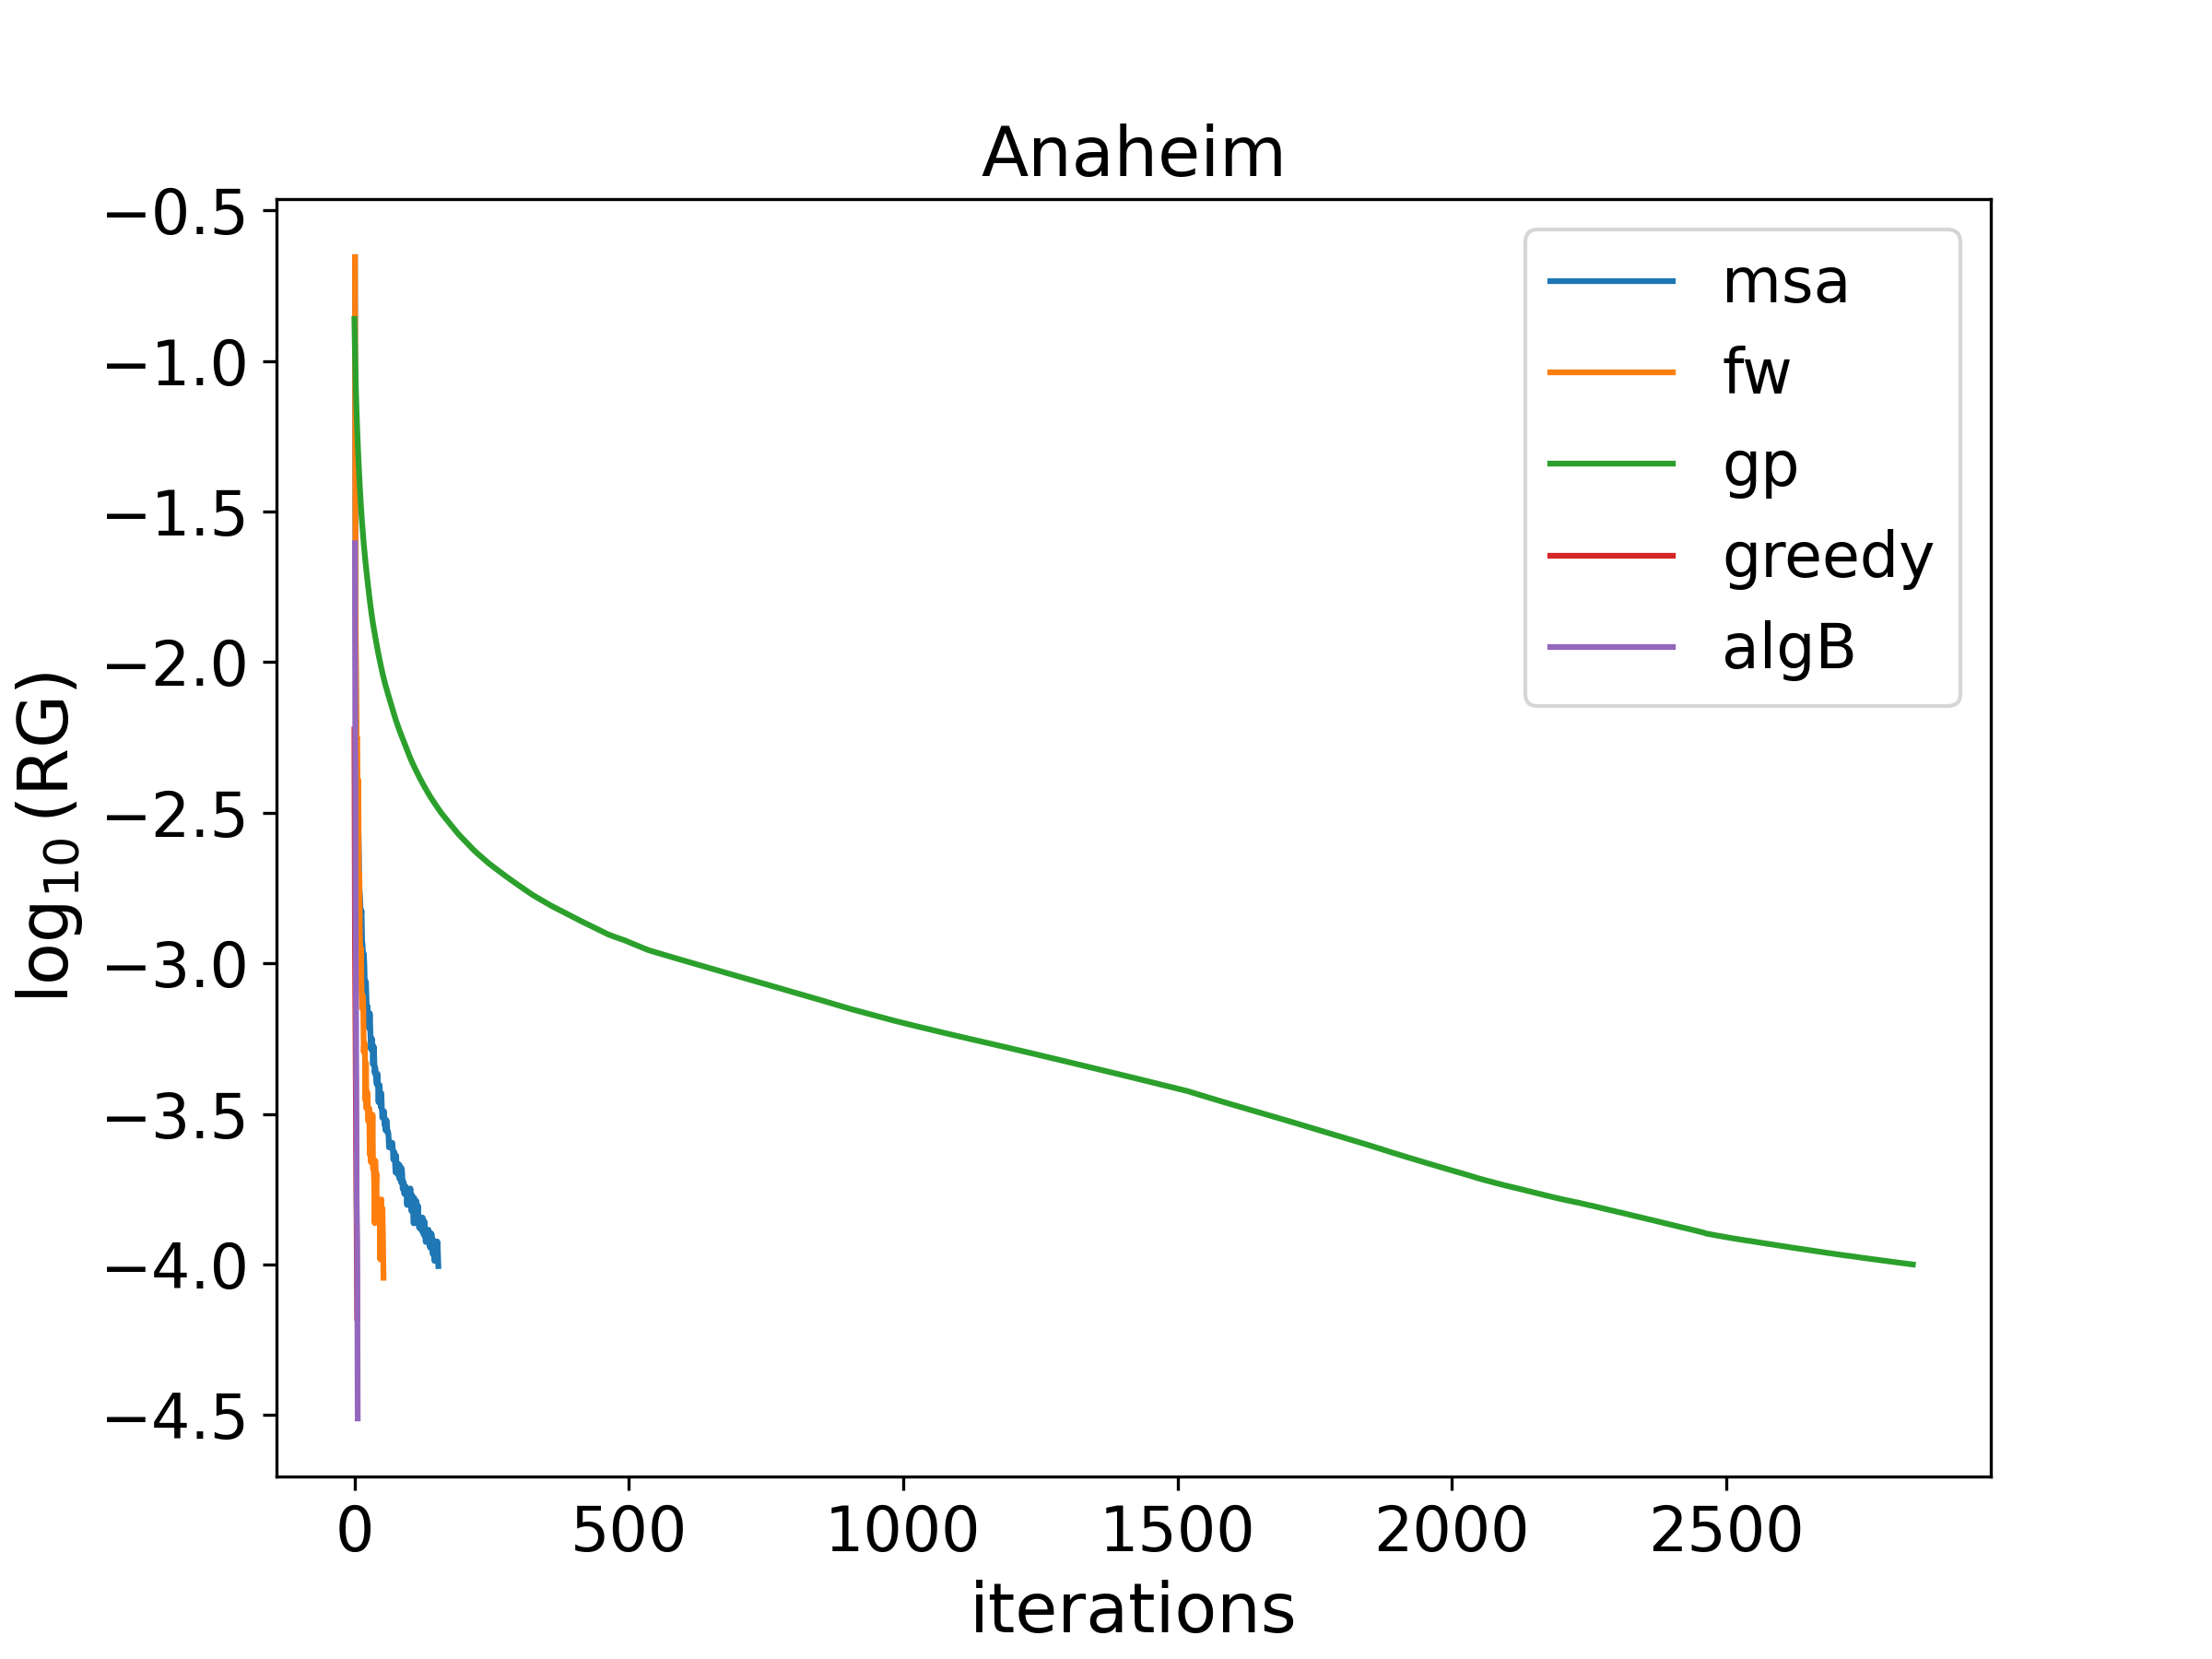
\includegraphics[width=\textwidth]{figures/Anaheim.png}
\caption{Anaheim}
\end{subfigure}
\hfill
\begin{subfigure}{0.5\linewidth}
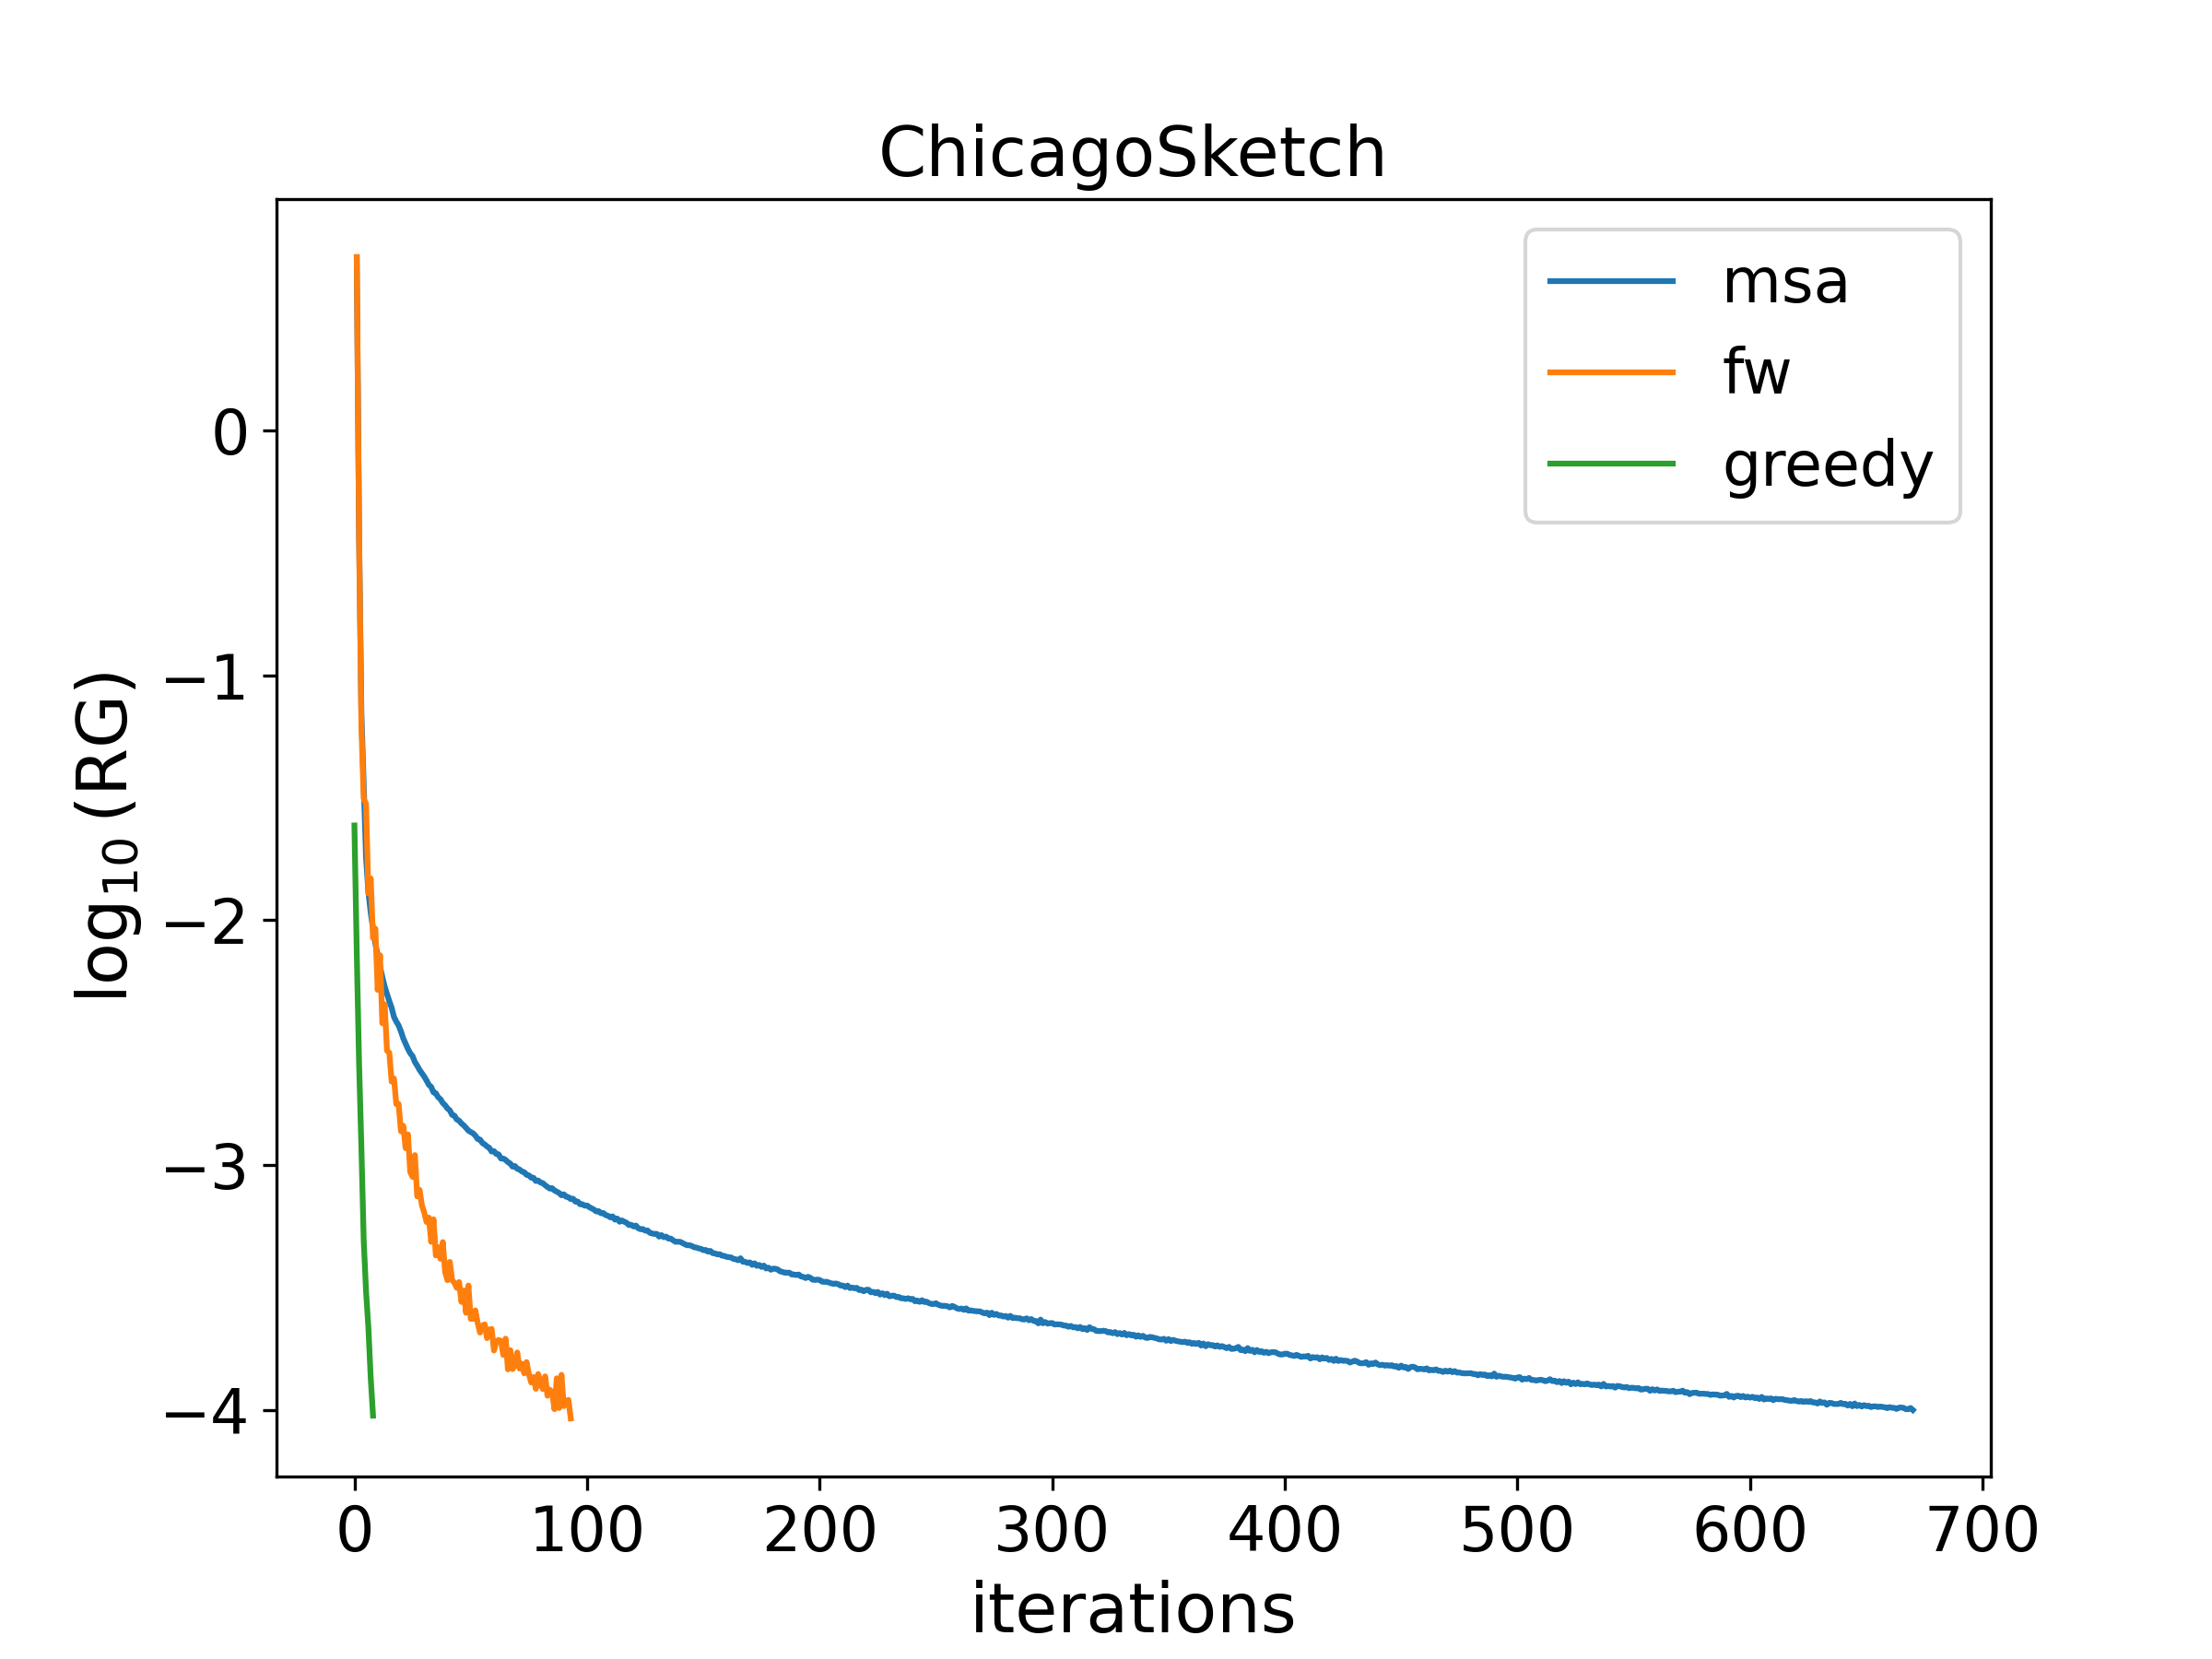
\includegraphics[width=\textwidth]{figures/ChicagoSketch.png}
\caption{Chicago Sketch}
\end{subfigure}
\hfill
\begin{subfigure}{0.5\linewidth}
\centering
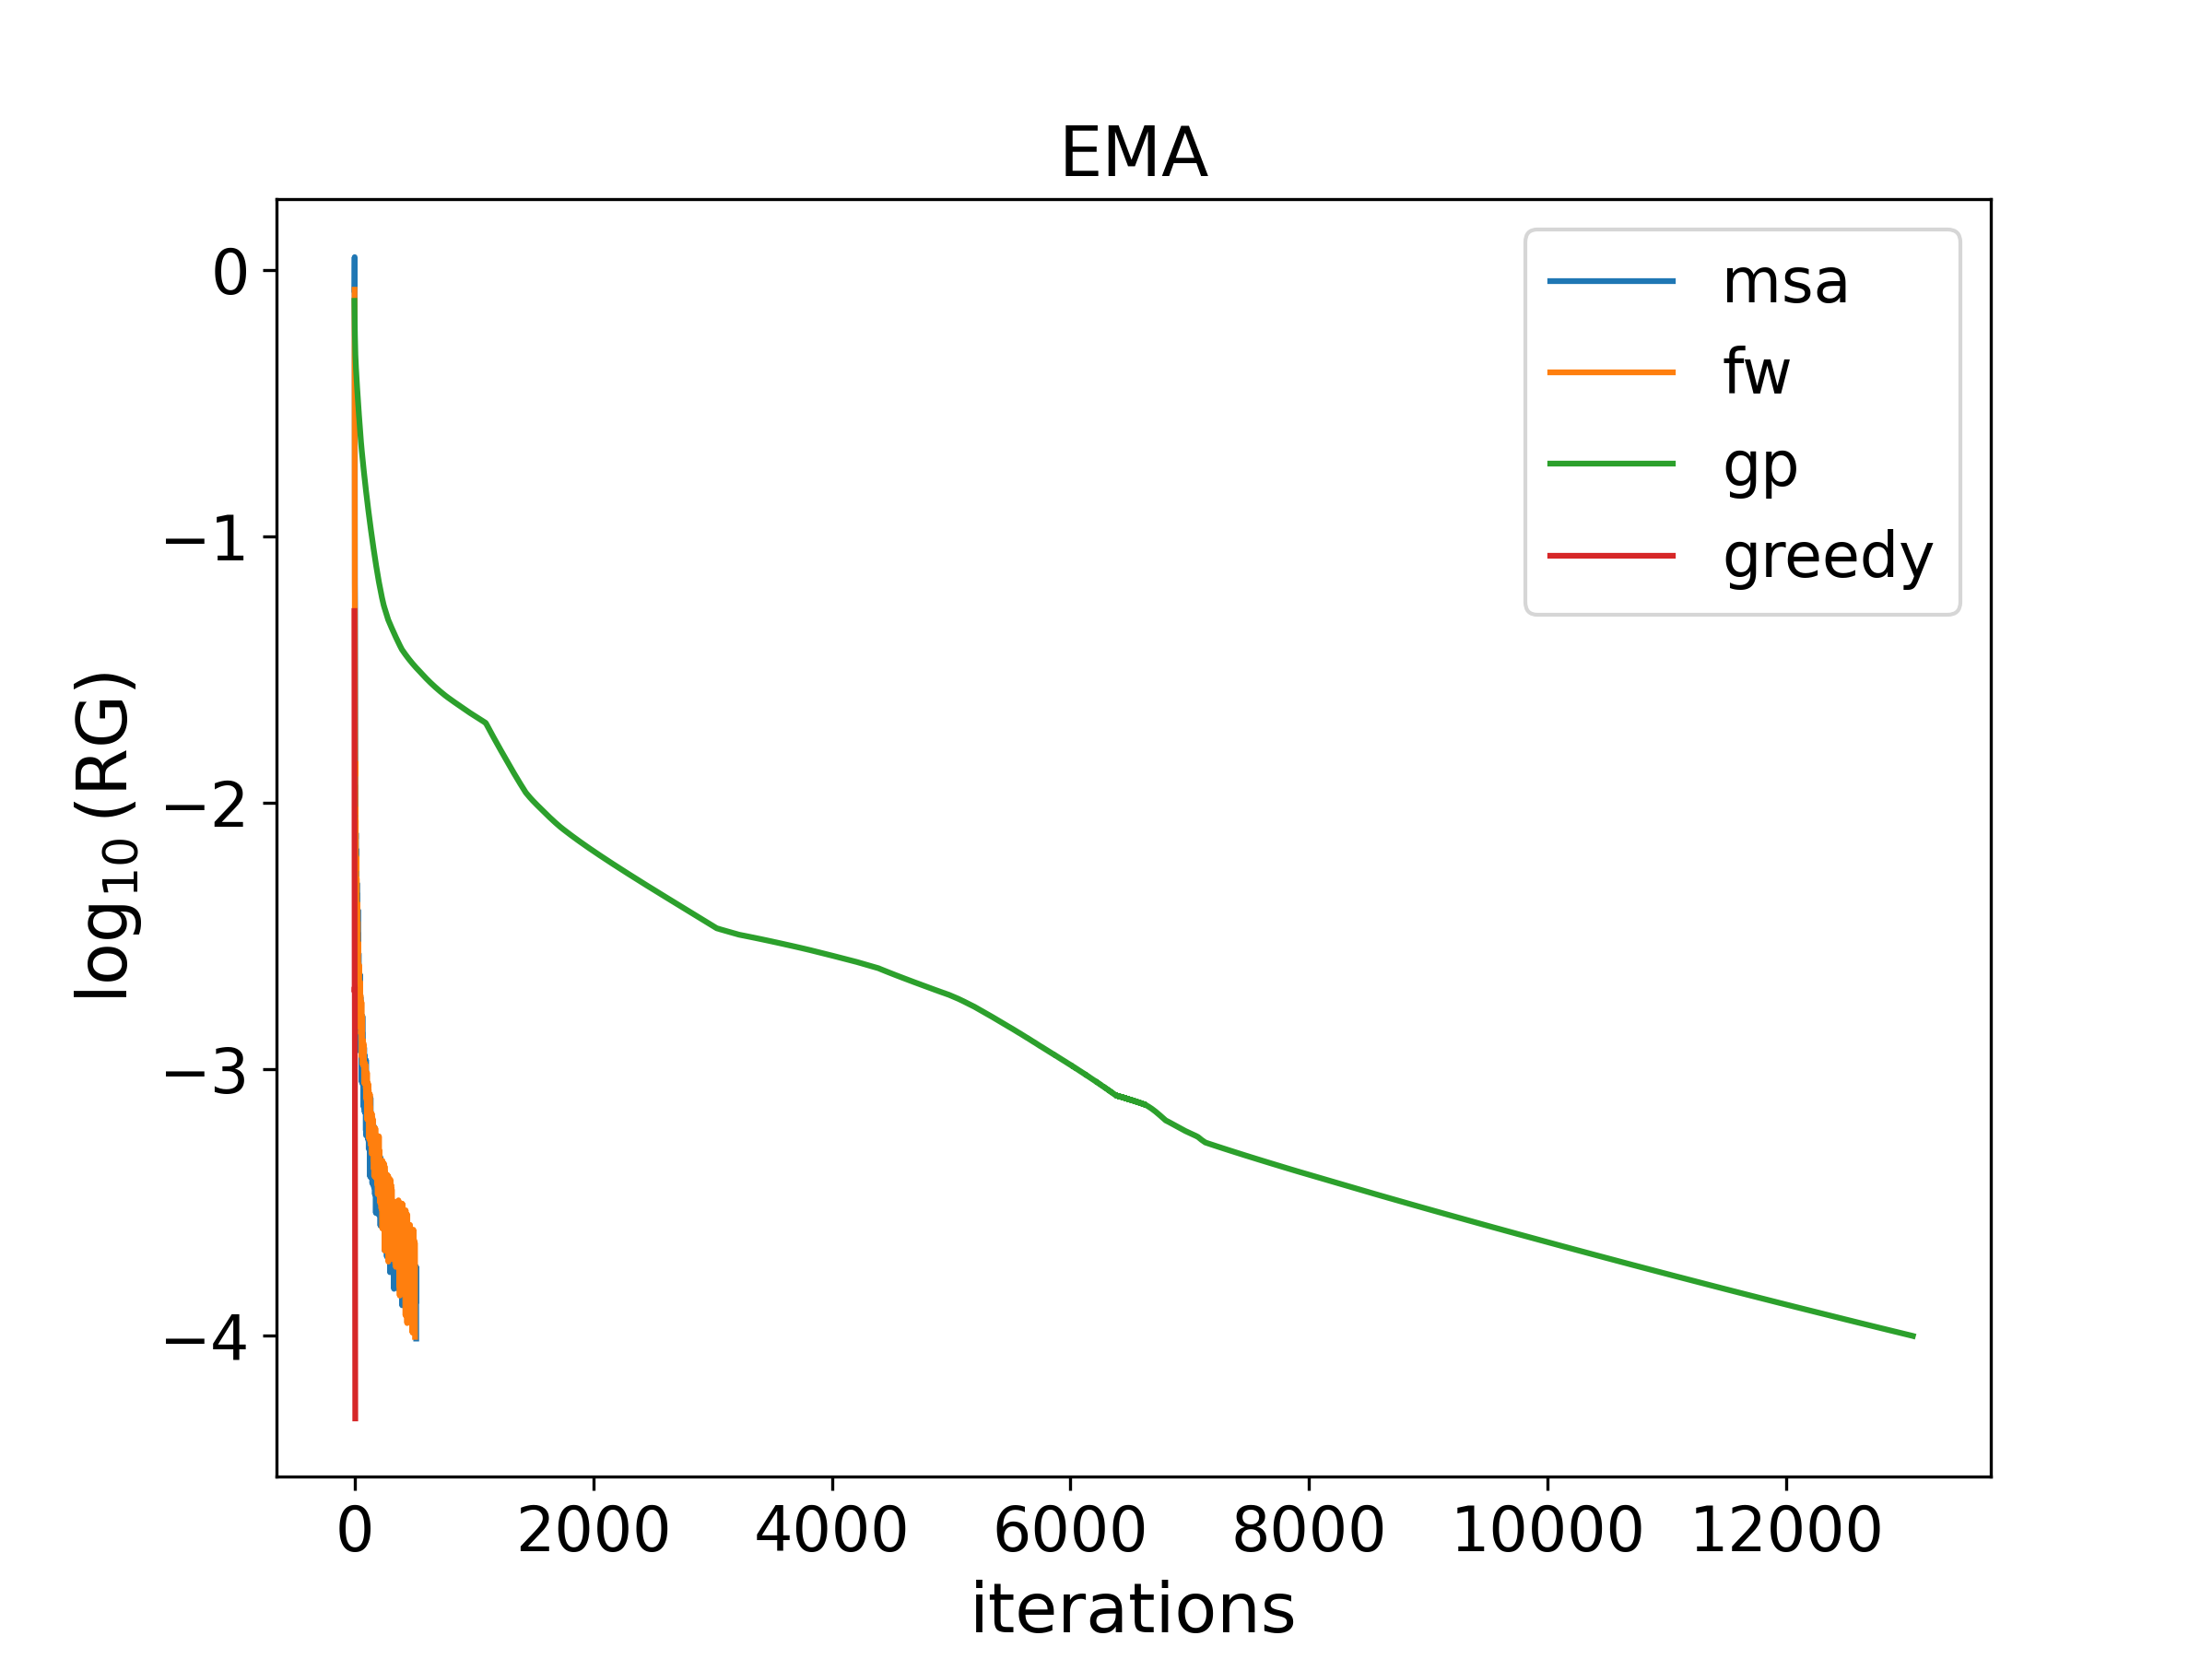
\includegraphics[width=\textwidth]{figures/EMA.png}
\caption{Eastern Massachusetts}
\end{subfigure}
\hfill
\begin{subfigure}{0.5\linewidth}
\centering
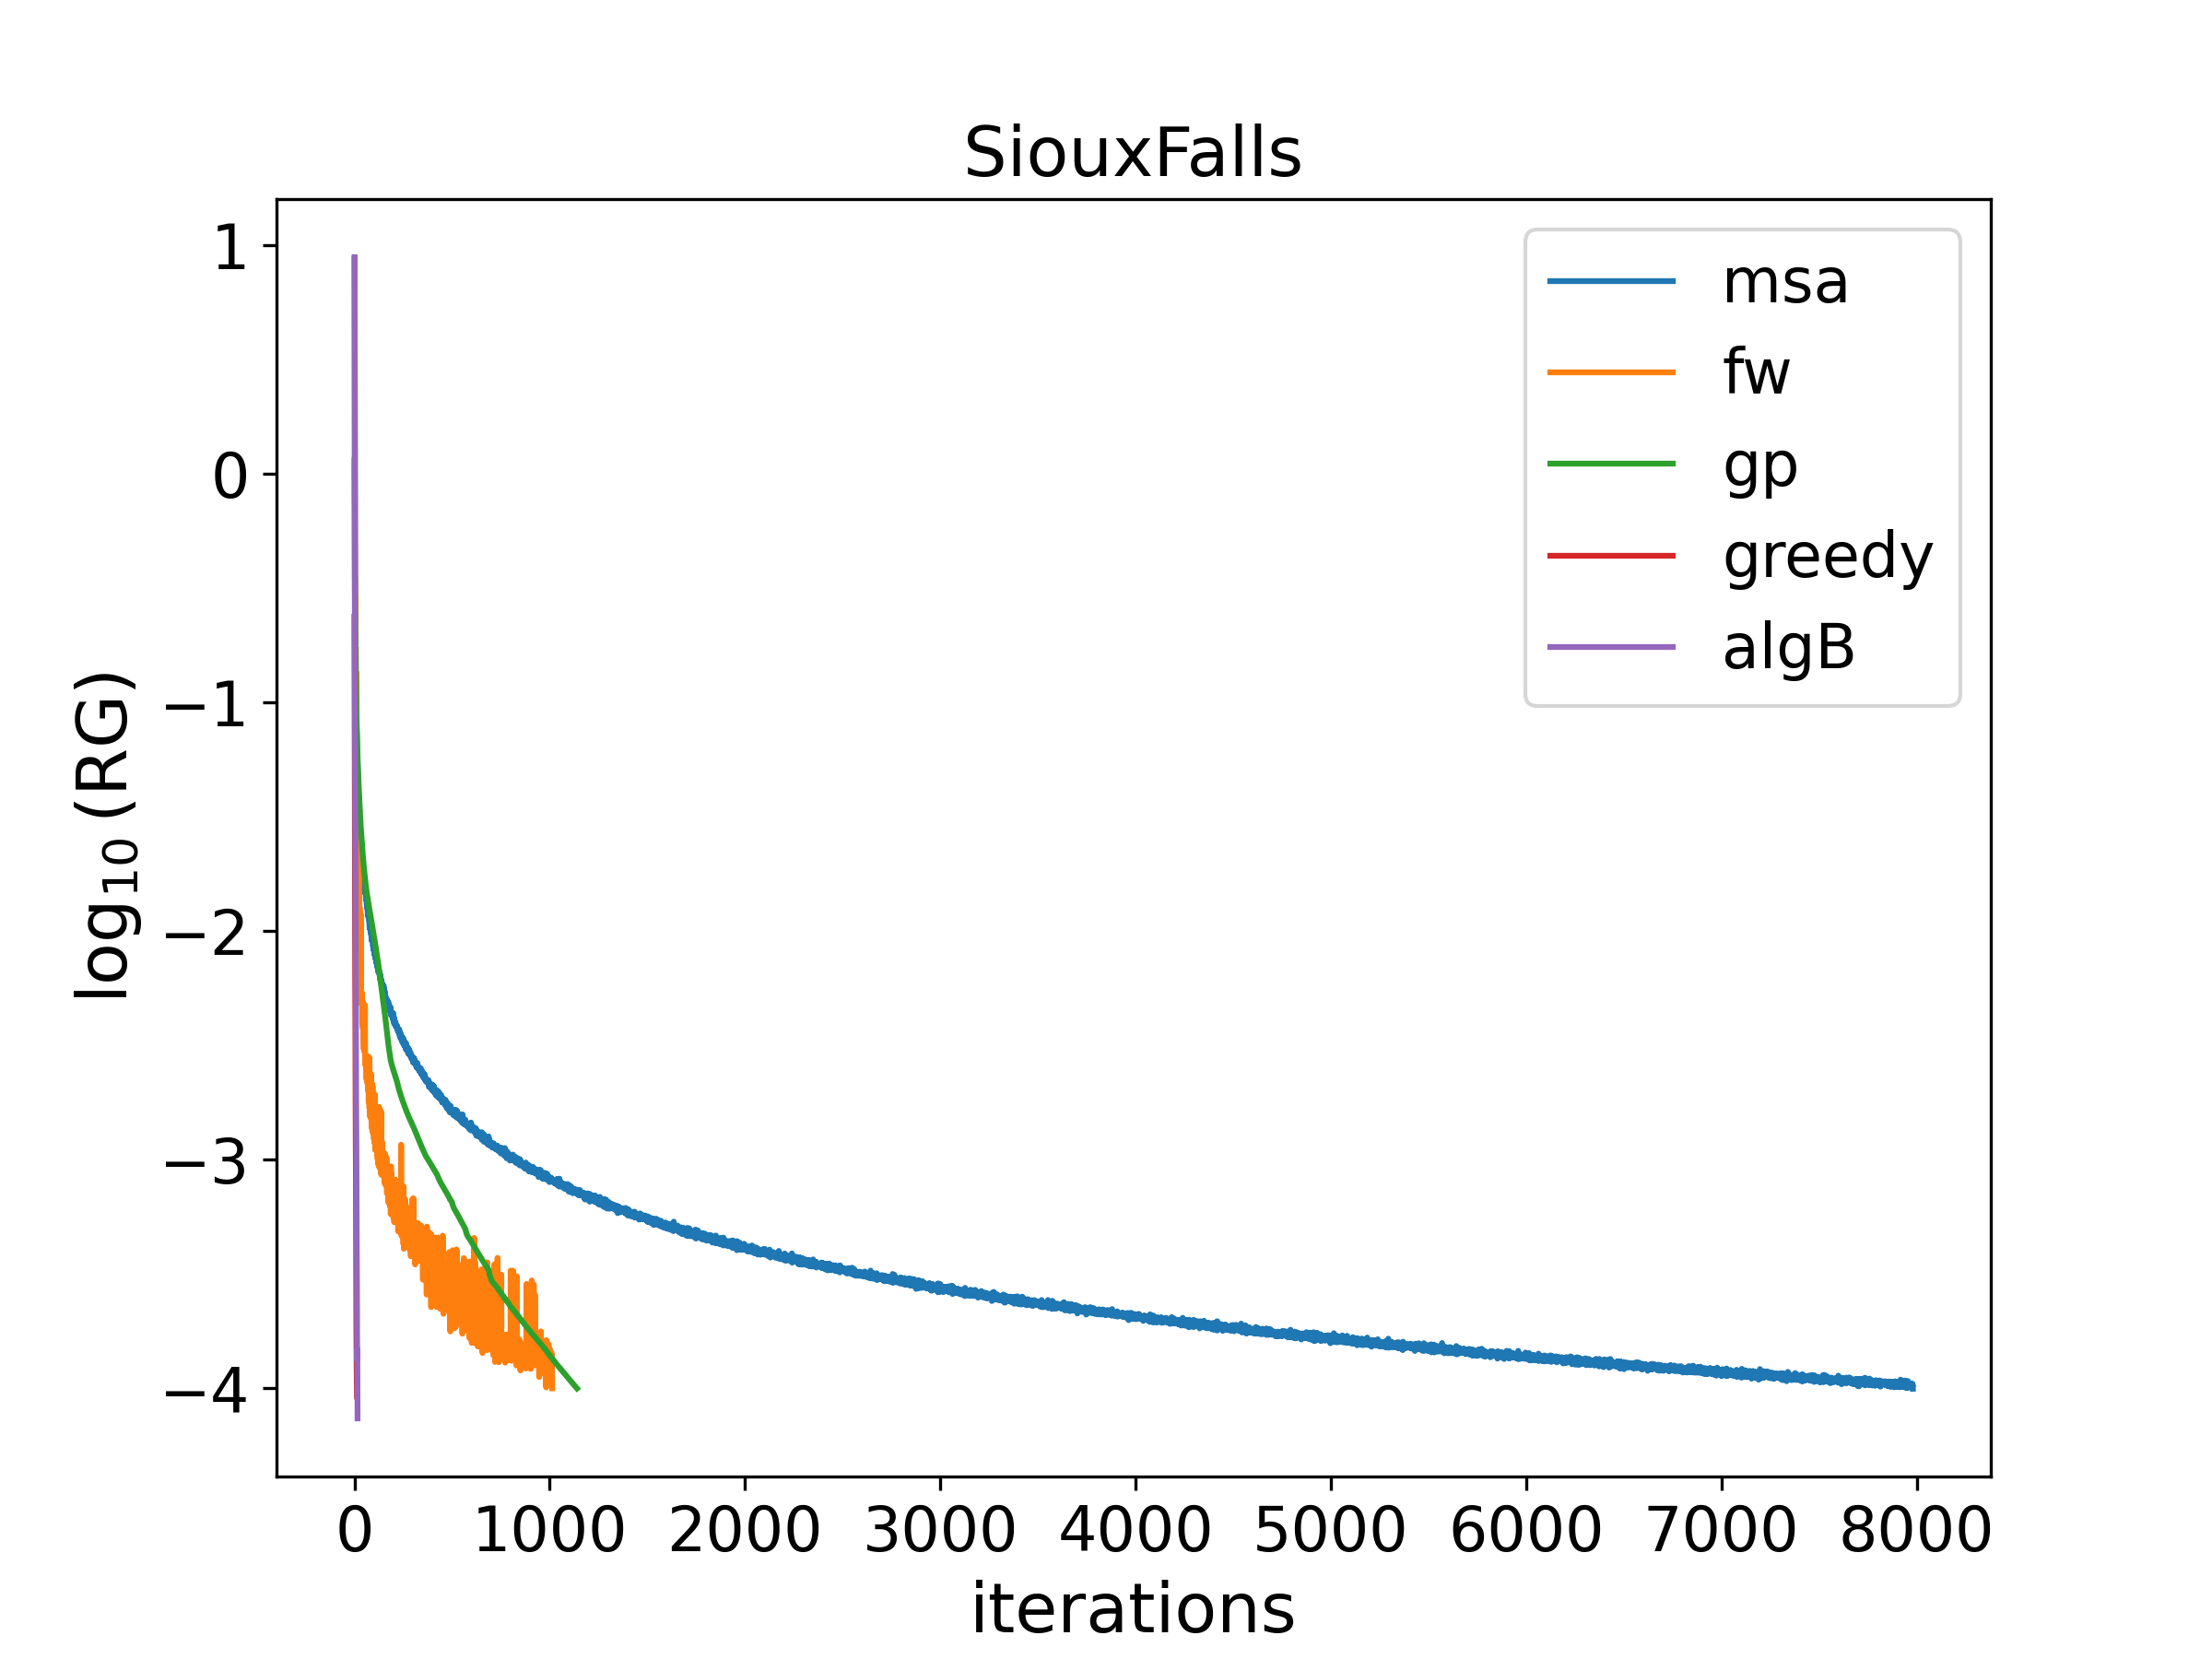
\includegraphics[width=\textwidth]{figures/SiouxFalls.png}
\caption{Sioux Falls}
\end{subfigure}
\label{plots}
\end{figure}



\section{Conclusions}
From the experimental data, the greedy algorithm clearly outperforms
other algorithms.
But for large networks, the python implementation
failed to give results within reasonable amount of time.
This limitation was overcome by the C++ implementation.
